\section{OpenFOAM}
%
Las flujometrías se realizaron con \emph{OpenFOAM}, un software de
Fluidodinámica Computacional, o CFD por sus siglas en inglés, de código libre y
abierto escrito en ``C++''.
%
% La herramienta seleccionada para realizar las flujometrías es OpenFOAM, por ser
% una herramienta libre y de código abierto.
%
Junto con este programa se utilizaron otras herramientas libres para generar la
geometría a modelar y post-procesar los resultados..
%
\subsection{Metodología}
%
El esquema de trabajo para realizar las simulaciones consistió en:

\begin{enumerate}
        %
    \item Pre-procesado
      %
        \begin{enumerate}
                %
            \item Definir la geometría a analizar.
              %
            \item Generar una malla con un tamaño de elemento adecuado, la
                solución a problemas de CFD depende fuertemente de la cantidad
                y tamaño de celdas utilizadas.
              %
            \item Seleccionar los modelos adecuados.
              %
            \item Definir las propiedades del fluido.
              %
            \item Definir las condiciones de borde.

              %
        \end{enumerate}
        %
    \item Solver
      %
    \begin{enumerate} \item Seleccionar el solver a utilizar.
            %
            \item Ejecutar la simulación.
            %
    \end{enumerate}
        %
\item Post-procesado
      %
    \begin{enumerate}
                %
        \item Visualizar los resultados de las distintas variables de la
            simulación.
            %
        \item Extraer la información necesaria.
            %
    \end{enumerate}
        %
\end{enumerate}

%%%%%%%%%%%%%%%%%%%%%%%%%%%%%%%%%%%%%%%%%%%%%%%%%%%%%%%%%%%%%%%%%%%%%%%%%%%%%%%

\subsection{Configuración}
%
Para configurar una simulación de OpenFOAM se configura el directorio de
simiulación como se indica en la figura XXX y XXX, cada directorio contiene una
carpeta con condiciones iniciales ``0'', malla ``constant'' y configuraciones
particulares de cada solver ``system''.

En el directorio ``0'' se dejan las condiciones iniciales y de borde de cada
simulación, utilizando una configuración genérica con parámetros definidos en un
archivo con los valores de condiciones iniciales, aprovechando las
características paramétricas de OpenFOAM, que permite corridas de una gran
cantidad de simulaciones en serie.

Estos archivos de condicinoes inciiales se generan con un \emph{script} que toma
valores de las simulaciones de \emph{ICESym}, como se indicó en la
sección~\ref{cap2:cond_iniciales}, en la que también se detallan las ecuaciones
e hipótesis utilizadas para obtener dichos valores.
%
La ejecución de las simulaciones también se automatizan con scripts de
\emph{bash} con los pasos para ejecutar las corridas con \emph{ICESym}.
%
Con los resultados de las simulaciones se procede a calcular/leer la magnitud
del caudal másico, necesario para el cálculo del coeficiente de descarga.

\subsubsection{Pre procesado}
%
El preprocesado consiste en definir geometría y condiciones iniciales, los datos
de partida  se obtienen de las simulaciones con ICESym.
%
Con los resultados del simulador se grafica la diferencia de presión entre
el puerto de admisión o escape y la cámara de combustión en función de
la apertura del puerto para velocidades de 1000 RPM a 9000 RPM.
%
Un ejemplo de esto se puede ver en la figura~\ref{fig:puntos_interes}, como
es de esperarse se tienen mayores diferenciales de presión a manores aperturas
del puerto porque para estas alzadas se está en la apertura o cierre del mismo.

A diferencia del puerto de admisión, en el puerto de escape se ve una banda
bastante definida de operación que se hace más ``llena'' a medida que se abre el
puerto.
%
Durante la apertura del puerto se ven las mayores diferencias de presión en las
que hay dos bandas bien definidas, se toman algunos puntos arriba en la zona con
mayor $\Delta P$ y una cantidad menor para velocidades con $\Delta P = 0$.
%
A medida que el puerto se abre la diferencia de presión con el gas en la cámara
de combustión se equaliza y esta banda se afina, requiriendo menos puntos para
caracterizar el funcionamiento de los mismos.

\begin{figure}
    \centering
    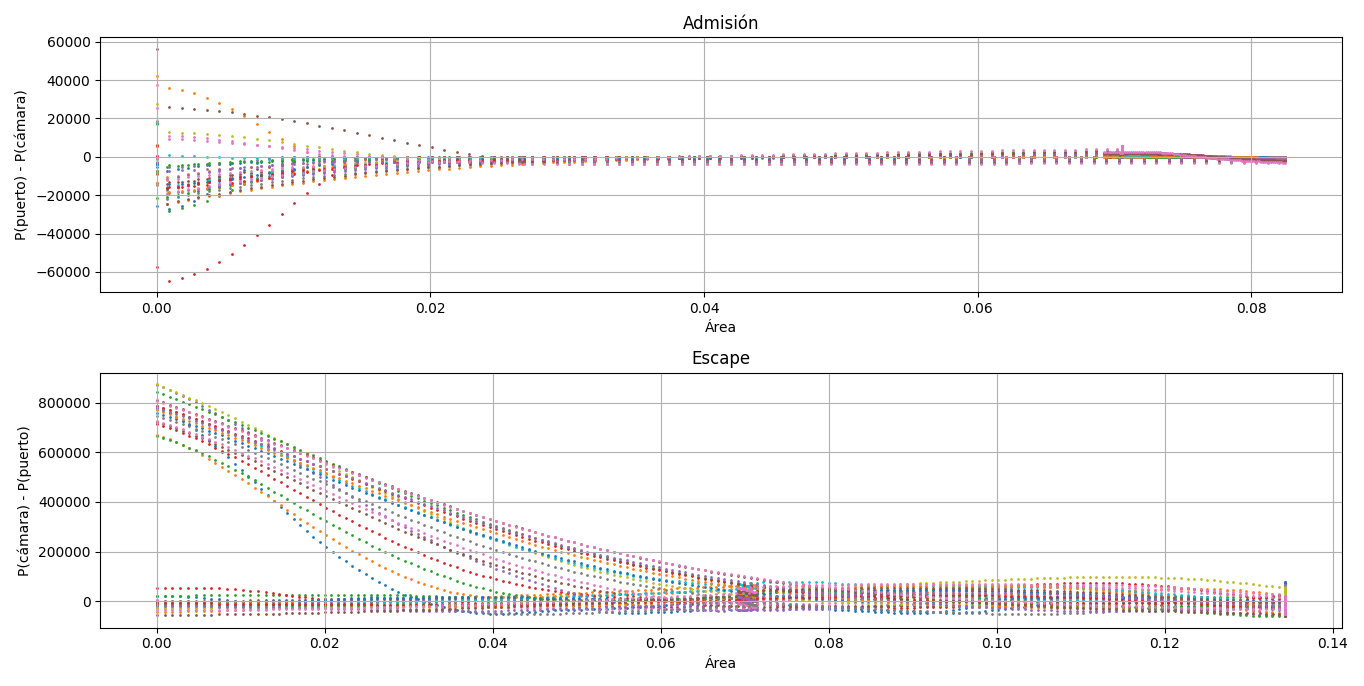
\includegraphics[width=\textwidth]{flujometrias/puntos_de_interes.png}
    \caption{Presión en función de la apertura el puerto,
$\Delta P = f(l_{v})$}\label{fig:puntos_interes}
\end{figure}

% Se definió el dominio de la simulación a partir de la geometría obtenida de
% la optimización con el algoritmo genético del motor utilizando coeficientes
% de descarga constantes para el flujo a través de los puertos.
%
El valor de alzada está directamente relacionado con el la posición angular del
cigüeñal, por lo que una vez seleccionados los puntos de interés se puede
extraer la geometría deseada de un modelo de CAD paramétrico del motor.
%
Este modelo tiene solamente la mitad que contiene los puertos de admisión y
escape, se obtuvo realizando operaciones geométricas con los volúmenes que
representan diferentes componentes del motor como son el estator, rotor,
paletas, etc.
%
En la figura~\ref{fig:admision_50} se muestra parte del proceso para obtener el
puerto de admisión a $\theta=50^{\circ}$, en donde se suma el volumen del mismo
en gris y las figuras que se restan que corresponden al rotor, las paletas y un
paralelogramo para quitar una región que no se simuló.

\begin{figure}
    \centering
    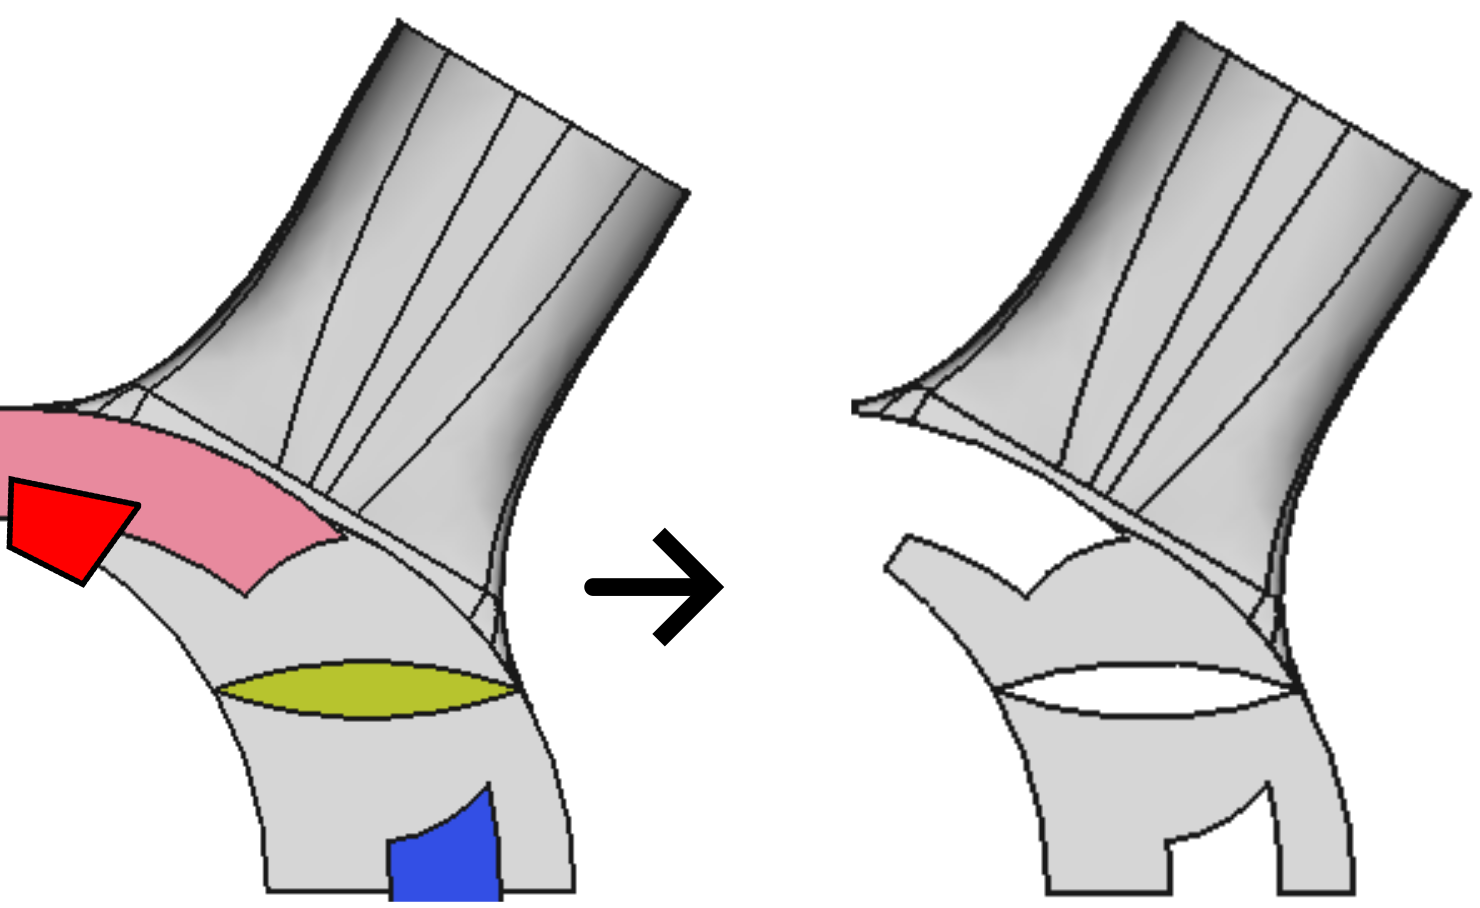
\includegraphics[width=0.7\textwidth]{./CAD/freecad_pasos.png}
    \caption{Puerto de admisión $\theta=50^{\circ}$Modelado con
FreeCAD}\label{fig:admision_50}
\end{figure}

Esta geometría fue generada por el programa FreeCAD~\parencite{freecad},
exportada a un archivo
``.BREP''\footnote{\href{https://dev.opencascade.org/doc/overview/html/specification\_\_brep\_format.html}{Formato
BREP, opencascade.org}} para luego ser importada en Salome\parencite{salome},
%
Salome se utiliza para generar una malla cerrada, hermética para que pueda ser
procesada por los complementos de OpenFOAM utilizados para generar la malla de
la simulación.
%
Es importante que la hermeticidad de la malla, esto significa que los nodos en
la frontera entre superficies coincidan, como se ve en la
figura~\ref{fig:salome_malla_hermetica}, en la que se ven dos superficies
"walls" y "outlet" y los nodos compartidos entre ambas superficies.
%
% Esto es así porque SnappyHexMesh parte de una malla como la generada por
% BlockMesh y la intersección de la misma con la superficie de un archivo".stl"
% (entre otros formatos).
%
% Se debe indicar un punto dentro o fuera de esta superficie \emph{stl},
% dependiendo del lado/cara por la que va a simularse el flujo, esto varía si un
% flujo externo o interno a la geometría.
%
% En este trabajo todos los flujos son internos por lo que se define una caja que
% encierra la totalidad del volumen de la malla \emph{stl} creada por Salome.

\begin{figure}
    \centering
    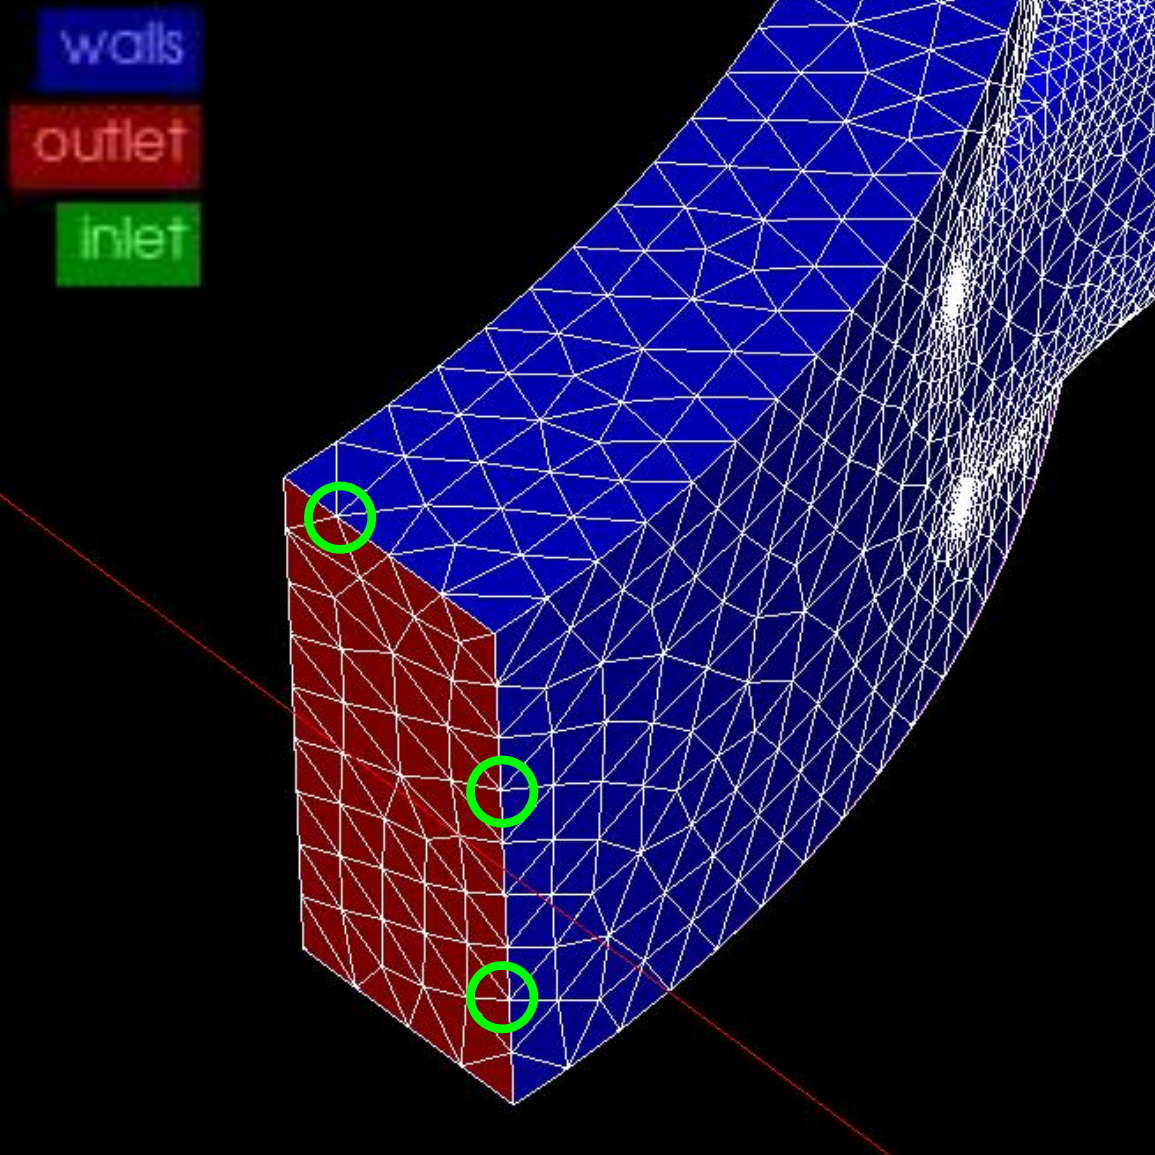
\includegraphics[width=0.5\textwidth]{./flujometrias/salome_malla_hermetica.png}
    \caption{Malla hermética}\label{fig:salome_malla_hermetica}
\end{figure}

El proceso en Salome consta de importar la geometría generada por FreeCAD y
separar la misma en superficies utilizadas para definir condiciones de contorno
en OpenFOAM, las superficies diferenciadas son: puerto, cámara/s, pared.

\begin{figure}
    \centering
    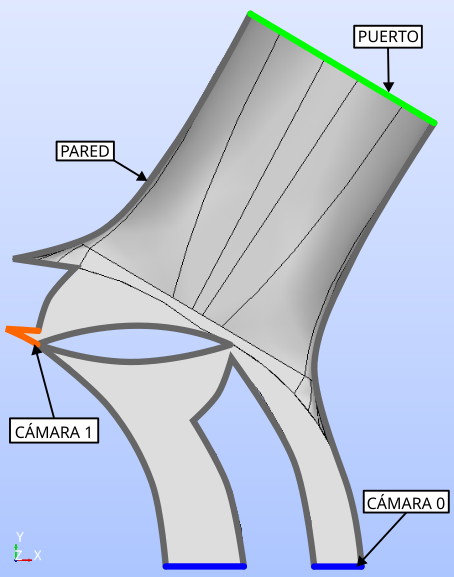
\includegraphics[width=0.7\textwidth]{./flujometrias/openfoam_parches.png}
    \caption{Nombres de Nombres de Parches}\label{fig:openfoam_parches}
\end{figure}

Luego de separadas estas superficies se procede a generar la malla en formato
ASCII STL con el complemento de mallado de Salome.
%
Se utilizó el generador de mallas NETGEN 1D-2D para crear la superficie, en
general se configuró el software de modo de tener un stl de buena calidad con
elementos de menor tamaño en zonas de mayor curvatura.
%
En la figura~\ref{fig:salome_fina_gruesa} se ve la diferencia en cantidad de
nodos de dos mallas, una malla fina a la izquierda y una malla gruesa a la
derecha.
%
En la tabla \ref{tab:salome_fina_gruesa} se muestra la diferencia entre algunos
parámetros básicos de configuración para las dos mallas.
%
% Esto sin requerir de una gran cantidad de elementos para no ralentizar el
% procesado con SnappyHexMesh.

\begin{figure}[t!]
    \centering
    \begin{subfigure}[t]{0.5\textwidth}
        \centering
        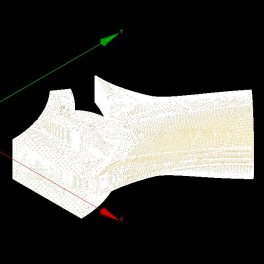
\includegraphics{/flujometrias/salome3_fina.png}
        \caption{Malla fina sin optimizar}
    \end{subfigure}%
    \begin{subfigure}[t]{0.5\textwidth}
        \centering
        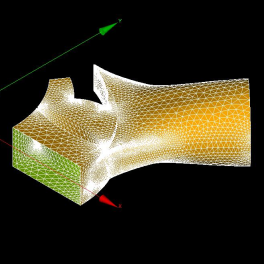
\includegraphics{/flujometrias/salome3_gruesa.png}
        \caption{Malla gruesa optimizada}
    \end{subfigure}
    \caption{Diferentes mallas para flujometrías}\label{fig:salome_fina_gruesa}
\end{figure}

\begin{table}
    \centering
    \begin{tabular}{lcc} \toprule
        Parámetro                & Malla Fina    & Malla Gruesa \\ \midrule
        Tamaño máximo            & 0.001         & 0.03 \\
        Tamaño mínimo            & 1E-7          & 2.4E-5 \\
        Limitado por curvatura   & Sí            & Sí \\
        Optimizar                & No            & Sí \\
        Cantidad de nodos        & 99311         & 49112 \\
        Cantidad de elementos    & 204695        & 103163 \\ \bottomrule
    \end{tabular}
    \caption{Configuración de mallas mostradas en la figura~\ref{fig:salome_fina_gruesa}}
    \label{tab:salome_fina_gruesa}
\end{table}

\subsubsection{Malla}
%
Una vez obtenido el archivo STL se procede a la generación de la malla dentro de
OpenFOAM con \emph{blockMesh} y \emph{snappyHexMesh}.
%
Primero se crea crea una malla con \emph{blockMesh} que  debe contener la
totalidad del volumen del puerto a simular, como se ve en la
figura~\ref{fig:paraview_blockMesh_stl}.
%
En este paso se define el tamaño de base de la malla y el nivel general de
refinamiento, a partir de estos cubos se produce el refinamiento por
\emph{castelación} que consiste en dividir las celdas en cubos más pequeños y luego
aplicar el \emph{snapping} para adaptarse a la superficie del volúmen que se está
modelando, ver figura~\ref{fig:openfoam_shm_pasos}.
%

\begin{figure}
    \centering
    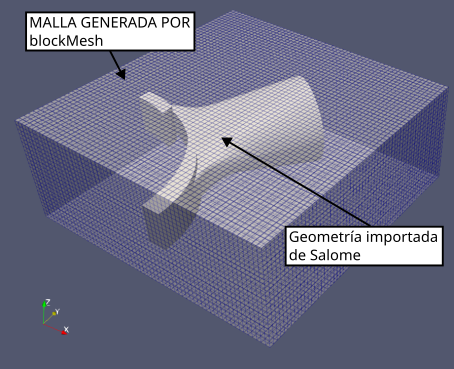
\includegraphics[width=0.5\textwidth]{flujometrias/paraview_blockMesh_stl.png}
    \caption{Malla de blockMesh y stl de Salome}\label{fig:paraview_blockMesh_stl}
\end{figure}

\begin{figure}[t!]
    \centering
    \begin{subfigure}[t]{0.5\textwidth}
        \centering
        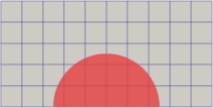
\includegraphics{flujometrias/shm_fondo.png}
        \caption{Malla de fondo y geometría}
    \end{subfigure}%
    \begin{subfigure}[t]{0.5\textwidth}
        \centering
        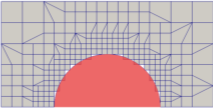
\includegraphics{flujometrias/shm_castelacion.png}
        \caption{Castelación}
    \end{subfigure}
    \begin{subfigure}[t]{0.5\textwidth}
        \centering
        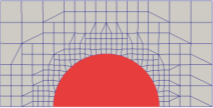
\includegraphics{flujometrias/shm_snapping.png}
        \caption{Snapping}
    \end{subfigure}
    \caption{Pasos de SnappyHexMesh\parencite{shm_steps}}\label{fig:openfoam_shm_pasos}
\end{figure}


\emph{blockMesh} crea una malla paramétrica con bloques con opción de gradientes
de tamaños y bordes curvados, los bordes pueden ser lineas rectas, arcos o
``splines''.
%
La malla se genera o configura con un diccionario \emph{blockMeshDict} ubicado
en \emph{constant/polyMesh}.

\emph{snappyHexMesh} es un generador de malla que toma una malla existente y la
\emph{talla} en la malla deseada, generando una malla 3D conformada por
hexaedors y hexaedros partidos a partir de superficies de caras triangulares en
formato de \emph{estereolitografía} (STL por sus siglas en inglés).
%
Además permite refinar zonas particulares de la geomeria y un refinamiento mayor
de la malla en la zona de la capa límite.


% %%%%%%%%%%%%%%%%%%%%%%%%%%%%%%%%%%%%%%%%%%%%%%%%%%%%%%%%%%%%%%%%%%%%%%%%%%%%%%%
% % NOTA: para esta sección, meter algo como lo que está aca abajo:
% % Para las flujometrías en las que no hay solape de cámaras, se definen las
% % propiedades de una entrada y una cámara de combustión, indicadas como
% % \emph{port} y \emph{chamber} respectivamente como se ve en la
% % figura~\ref{fig:ref_geom1}.
% % %
% % (Figura aca)

% % El puerto y la cámara de combustión (o cámaras en caso de que haya solape), se
% % definen como \emph{patch}, una frontera permeable.

% %%%%%%%%%%%%%%%%%%%%%%%%%%%%%%%%%%%%%%%%%%%%%%%%%%%%%%%%%%%%%%%%%%%%%%%%%%%%%%%
% \subsection{Coeficiente de descarga ($C_D$)}

% El coeficiente másico se calcula a partir de las ecuaciones de flujo
% compresible a través de una restricción, para el caso en que el flujo no esté
% bloqueado, la ecuación de $\dot{m}$ es:

% \begin{equation}
%     \label{eq:m_not_choked}
%     \dot{m} = \frac{C_D A_R p_0}{\sqrt{R T_0}}
%             {\left(\frac{p_T}{p_0} \right)}^{1/\gamma}
%             {\left( \frac{2\gamma}{\gamma-1} \left[1- {(\frac{p_T}{p_0})}^{{\gamma-1}/\gamma} \right] \right)}^{1/2}
% \end{equation}

% En caso del que el flujo esté bloqueado, es decir
% $p_T/p_0 \le {[2/\gamma+1]}^{\gamma/(\gamma - 1)}$
% , la ecuación correspondiente es:

% \begin{equation}
%   \dot{m}=  \frac {C_D A_R p_0} {{(R T_0)}^{1/2}}
%             \gamma^{1/2}
%             {\left( \frac{2\gamma}{\gamma+1} \right)}^{(\gamma+1)/(2(\gamma-1))}
% \end{equation}

% Para determinar $C_D$ se debe conocer:

% \begin{itemize}
%     \item $p_0$, es la presión de estancamiento antes de la restricción.
%     \item $T_0$, es la temperatura de estancamiento antes de la restricción.
%     \item $p_T$, es la presión estática justo después de la restricción.
%     \item $A_R$, es el área de referencia.
%     \item $\dot{m}$, es el caudal másico.
%     \item $\gamma$, es el cociente de capacidades térmicas del gas.
% \end{itemize}

% El área de referencia utilizada en ICESym es el área frontal del puerto expuesta
% a la cámara que se esté analizando, calculada como $A_{R} = h_{p} \cdot l_{{v}}$.
% %
% Debido a que el MRCVC no tiene válvulas, en trabajos anteriores se confeccionó
% un script para calcular la distancia $l_v$ en función del ángulo del ciclo.
% %
% En la figura~\ref{fig:area_referencia} se ilustran las áreas de referencia para
% una posición del rotor en la que hay solape de cámaras con $\theta = 55^\circ$.

% \begin{figure}
%     \centering
%     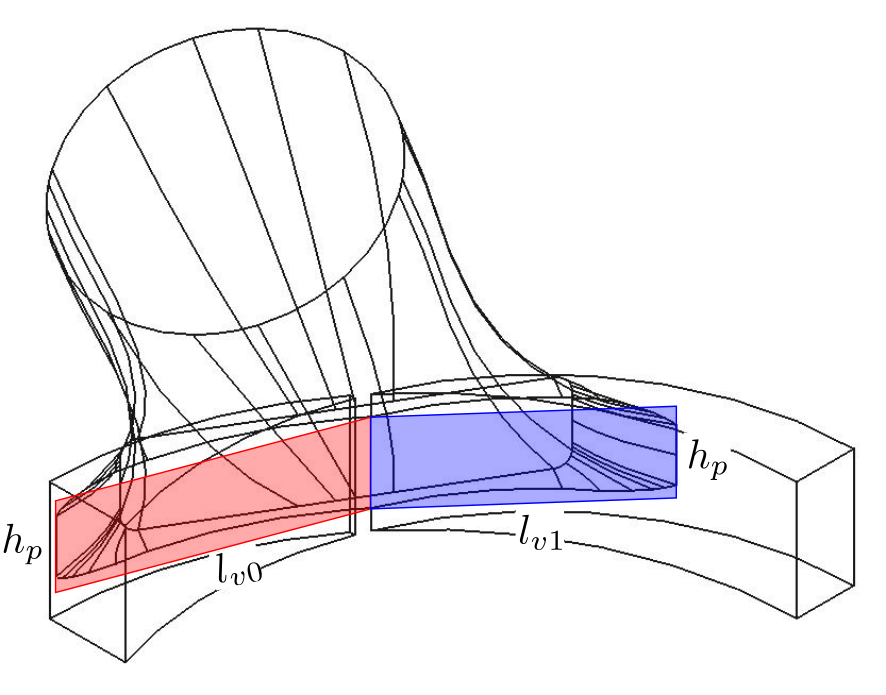
\includegraphics[]{area_referencia.png}
%     \caption{Área de referencia}\label{fig:area_referencia}
% \end{figure}

% Los valores de densidad, velocidad, presión y temperatura se obtienen de los
% datos de salida de ICESym para un puerto, ángulo y velocidad dada, en
% particular del archivo de salida con nombre \emph{$cyl_0.txt$} que contiene
% información relevante a la cámara de combustión.
% %
% Para la temperatura se utiliza la temperatura de cámara, $T_0 = T_C$, la
% presión antes y después del puerto se selecciona de acuerdo al sentido de
% flujo, en caso de ser flujo hacia la cámara de combustión, la presión en el
% puerto se utiliza como inicial $P_0$ y la presión en la cámara es la
% aproximación a la presión en la restricción $P_T$.

% Para inicializar el campo de presión y densidades, se usa la media entre las
% cámaras que se estén simulando y se establece un campo uniforme.

% La velocidad se inicializa con un campo nulo de velocidades, que en la
% configuración de OpenFOAM se designa como \emph{internalField uniform (0 0 0)}.

% En resumen, los valores iniciales de los campos de presión, temperatura y velocidad
% son los indicados en la tabla~\ref{tab:cc}.

% \begin{table}
% \centering
%     \begin{tabular}{cccc} \toprule
%         Var & Campo         & Parche                      & Pared \\
%         T   & uniforme T0   & inletOutlet                 & uniforme T9\\ \midrule
%         P   & uniform Pavg  & uniformTotalPressure        & Pi \\
%         U   & uniform (0 0 0) & pressureInletOutletVelocity & valor fijo (0 0 0)\\
%         rho & uniform rhoAvg \\ \bottomrule
%     \end{tabular}
%     \caption{Condiciones de Borde}\label{tab:cc}
% \end{table}

% En todos los casos se tomará como velocidad de referencia a la media entre la
% velocidad en la punta del tubo de las cámaras solapadas.
% %
% Del mismo modo, la temperatura será la temperatura de cámara media.

% Si hay o no solape de cámaras va a depender tanto de la geometría del puerto
% como de la posición del ciclo en la que se encuentre, para determinar las
% condiciones iniciales se debe tener en cuenta el solape.
% %
% En la figura~\ref{fig:geom} se muestra un corte del puerto con un plano cuya
% normal está en $\vec{z}$, se denominará a la cámara que esté a la izquierda
% como cámara 0 y a la que esté a la derecha cámara 1
% %
% Al haber solape de cámaras, para definir la presión del puerto y estimar las
% condiciones iniciales de los parámetros viscosos que requiere el modelo
% $k-\epsilon$ se utilizan valores medios de presión, velocidad y temperatura de
% ambas cámaras.
% %
% Además, las condiciones iniciales de que se aplican al parche denominado
% \emph{puerto} es igual a la media aritmética de la velocidad de las velocidades
% de los puertos de ambas cámaras, Lo mismo sucede con la presión, densidad y
% temperatura.

% A partir de estos datos se calculan varias propiedades termodinámicas del gas,
% incluyendo la constante del gas, masa molar, viscosidad cinemática y demás.
% %
% Para calcular estas propiedades se asume que el gas no contiene gases
% residuales.

% Finalmente el caudal másico yse obtiene con OpenFOAM, en donde se simula el
% tiempo suficiente para que los caudales másicos por entradas o salidas se
% estabilice, como se ve en la figura~\ref{fig:caudalMasico}.

% \begin{figure}
%     \centering
%     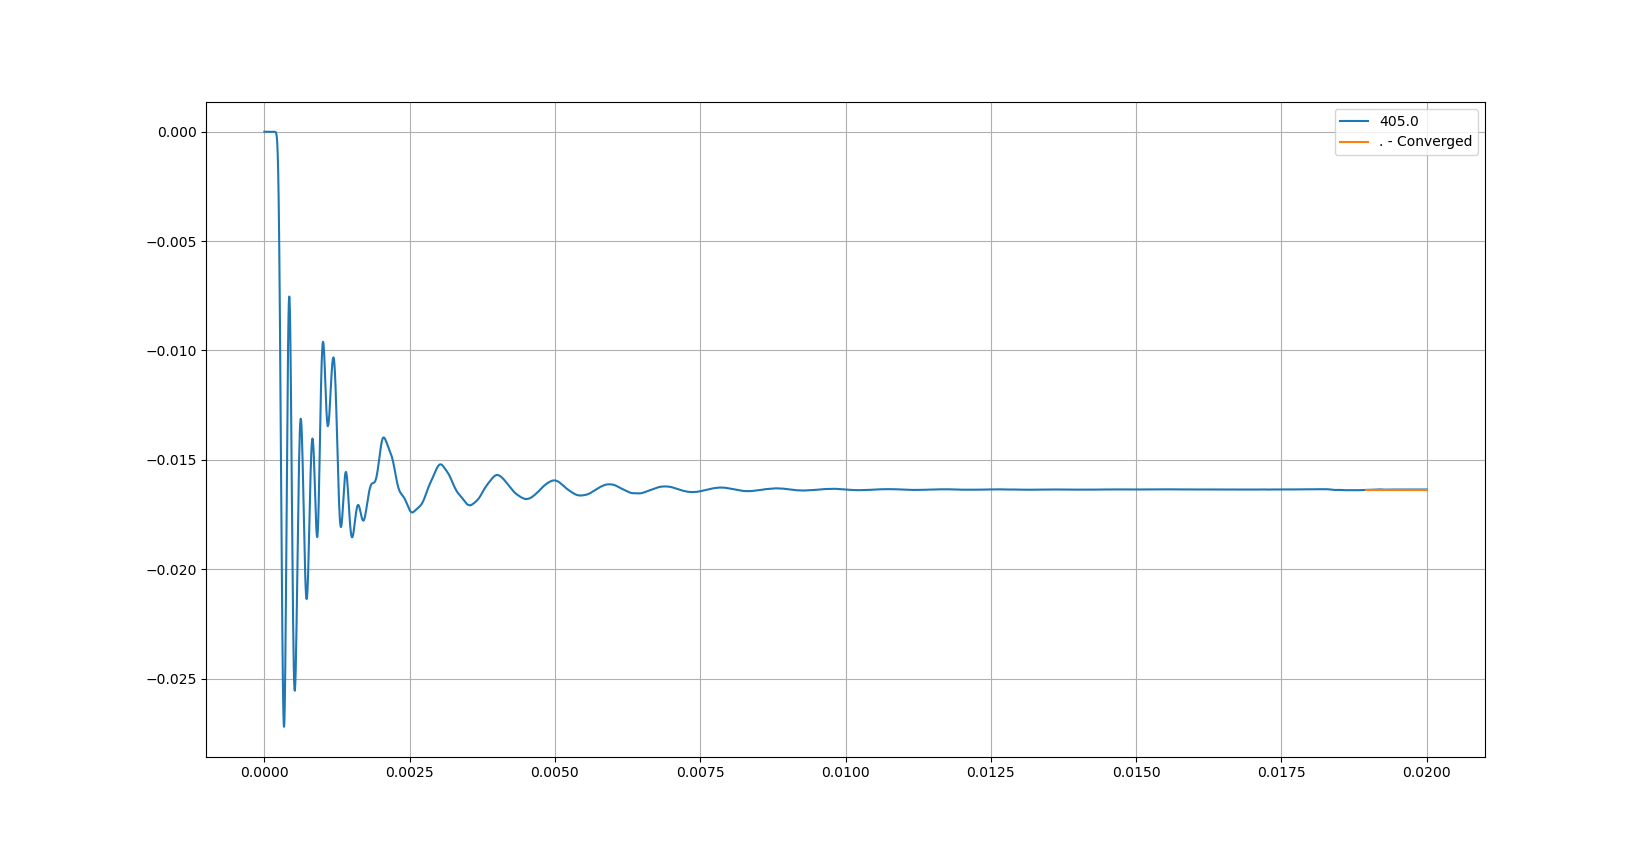
\includegraphics[width=0.6\textwidth]{surfaceFieldValue_405.0.png}
%     \caption{Flujometrías para el puerto de Admisión}\label{fig:caudalMasico}
% \end{figure}
% En todos los casos se tomará como velocidad de referencia a la media entre la
% velocidad en la punta del tubo de las cámaras que se estén solapando.
% %
% Del mismo modo, la temperatura será la temperatura de cámara media.

% Si hay o no solape de cámaras va a depender tanto de la geometría del puerto
% como de la posición del ciclo en la que se encuentre, para determinar las
% condiciones iniciales se debe tener en cuenta el solape.
% %
% En la figura~\ref{fig:geom} se muestra un corte del puerto con un plano cuya
% normal está en $\vec{z}$, se denominará a la cámara que esté a la izquierda
% como cámara 0 y a la que esté a la derecha cámara 1
% %
% Al haber solape de cámaras, para definir la presión del puerto y estimar las
% condiciones iniciales de los parámetros viscosos que requiere el modelo
% $k-\epsilon$ se utilizan valores medios de presión, velocidad y temperatura de
% ambas cámaras.
% %
% Además, las condiciones iniciales de que se aplican al parche denominado
% \emph{puerto} es igual a la media aritmética de la velocidad de las velocidades
% de los puertos de ambas cámaras, Lo mismo sucede con la presión, densidad y
% temperatura.


% %%%%%%%%%%%%%%%%%%%%%%%%%%%%%%%%%%%%%%%%%%%%%%%%%%%%%%%%%%%%%%%%%%%%%%%%%%%%%%%

% OpenFOAM is a free, open source computational fluid dynamics (CFD) software
% package released by the OpenFOAM Foundation.
% %
% It has a large user base across most areas of engineering and science, from both
% commercial and academic organisations.
% %
% OpenFOAM has an extensive range of features to solve anything from complex fluid
% flows involving chemical reactions, turbulence and heat transfer, to solid
% dynamics and electromagnetics.
